\subsection*{Jak se vaří na táboře} % (fold)
\label{sub:jak_se_vaří_na_táboře}

% subsection jak_se_vaří_na_táboře (end)

Opuchlé oči od kouře, pořezané prsty, ranní vstávání a neustálé počítání, odhadování nebo používání metody pokus – omyl. Ano, zasvěcení už tuší, tohle bude článek o táborové kuchyni.

Co vám budu povídat, vaření může být zábava, ale po třech týdnech živení spousty malých hladových krků (a pár uďovských) už máte na zbytek roku kuchtění dost. Pro vás, kteří stále netuší, co takové šéfování táborové kuchyni obnáší, mám shrnutí těch nejzajímavějších zážitků. 


Mezi těmi nejlepšími určitě nesmí chybět smažení řízků na závěrečnou popokladovkovou hostinu. Až si jednou řeknete, že udělat dětem radost touhle dobrotou je super nápad, tak vás musím varovat, není. Už jenom odhadnout počet řízků a nakoupit je byla celkem výzva a co teprve samotné krájení, obalování a smažení. Stojíte u hrnce, praží do vás současně sluníčko a oheň z kamen, pot z vás jen leje, jste popálení od prskajícího oleje a po první várce už musíte předat štafetu někomu jinému. Po pěti hodinách máte konečně hotovo všech 170 řízků a říkáte si, jestli to vůbec stálo za to. Třešničkou na dortu pak bylo zjištění, že by nám jich stačila tak polovina. Ale což, na uďovině přišly také vhod a hlavně že děti měly radost, ne?

Za zmínku stojí i připravování anglické snídaně. To jsme měly s Pískletem další skvělý nápad, jak náš jídelníček trochu ozvláštnit, a kdyby si Pískle neupustila sekeru na hlavu a nebyla na pár dní lehce indisponovaná, určitě by to byla velmi kvalitní ranní párty. Takhle to sice taky byla párty, ale pro příště asi zůstaneme u klasického poridge. Ono po ránu se snažit vymyslet, jak osmažit na našich kamnech slaninu nebo opéct tousty není úplně jednoduché a zapojit do toho skupinku službících Urzonů už je vyloženě stresující.

Nejvtipnější okamžik zcela jistě nastal ve chvíli, kdy jsme napsaly do seznamu nákupu, netušíc nic zlého, celer do polívky. Ani ve snu by nás nenapadlo takovou položku nějak víc zkonkretizovat, popsat, připojit obrázek nebo jinak upřesnit. Namísto klasické celerové bulvy se nám však z nákupu vrátily pouze celerové listy a popravdě trvalo velmi dlouho, než jsme pochopily, co že to má být. Po dlouhém a lehce hysterickém smíchu jsme „celer“ odložily do sklípku s tím, že se snad pro něj najde nějaké využití (nenašlo). 

\begin{center}

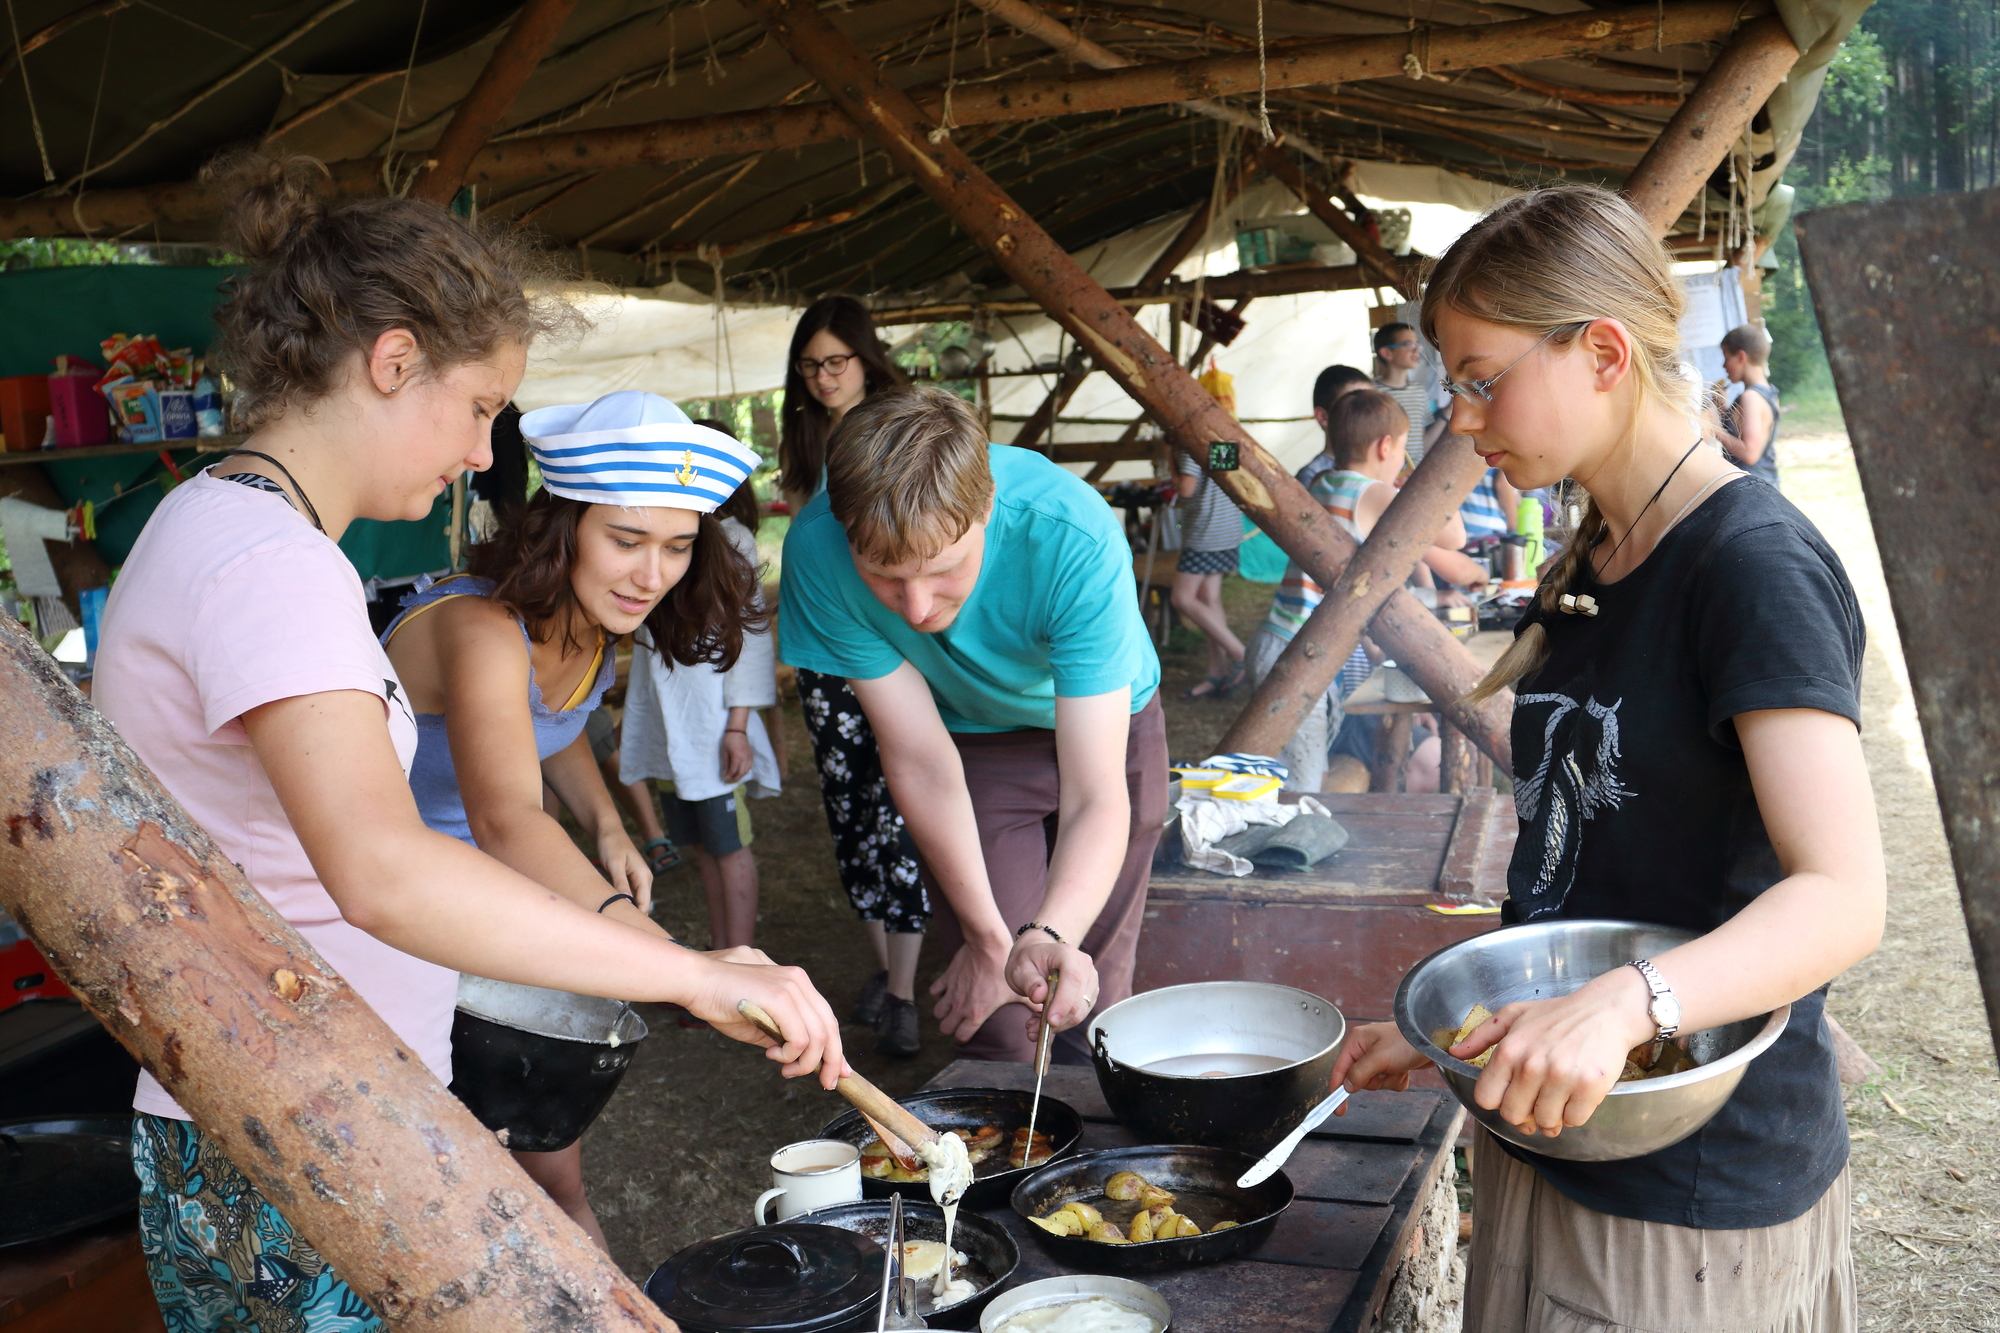
\includegraphics[width=12cm]{img/udo_clanky/kuchyne1.JPG}

\end{center}



Táborová kuchyně skýtá mnoho možností zažít věci, které si budete pamatovat po zbytek života. Jak jsme jedli celý den jenom zeleninu, jak nám myši spapaly svačinu nebo rozsekávání melounu mačetou jako nindža (přitom se mimochodem skvěle vybíjí jakákoliv frustrace). Klidně bych zvládla popsat střípky z kuchyně celou Knihu Keya, ale nechme tu prostor i pro další. Důležité je, že se zatím nikdo nepřiotrávil a všichni naše gastronomické výtvory ve zdraví přežili. 
\podpis{Kometa}

